\documentclass{scrartcl}
\usepackage[citestyle=authoryear,bibstyle=authoryear]{biblatex}
\addbibresource{bibliography}
\usepackage[utf8]{inputenc}
\usepackage[T1]{fontenc}

\usepackage{graphicx}
\graphicspath{{./figs/}}
\DeclareGraphicsExtensions{.pdf,.jpeg,.png,.eps}
\usepackage{amsmath}
\usepackage{amssymb}
\usepackage{amsthm}
\theoremstyle{definition}
\newtheorem{definition}{Definition}[section]

\newtheorem{prop}{Proposition}

\usepackage{cleveref}
\usepackage{algorithmic}
\usepackage{array}
\usepackage{booktabs}
\usepackage{stfloats}
\usepackage[super]{nth}
% for inkscape images
\usepackage{xcolor}
\usepackage{tikz,pgf}

\makeatletter
\g@addto@macro\@floatboxreset\centering
\makeatother

% \usepackage{hyperref}
 
 \AtBeginDocument{% Overrides ref for Cref
 	\let\ref\Cref
 }

\begin{document}
% INPUT PREAMBLES
% # PAPER SPECIFIC
\global\long\def\Tsq{T^{2}}%
\global\long\def\priordist{p_{z}}%
\global\long\def\detencoding{g_{\mbphi}}%
\global\long\def\detdecoding{f_{\mbtheta}}%
\global\long\def\encoding{q_{\mbphi}(\mbz\g\mbx)}%
\global\long\def\decoding{p_{\mbtheta}(\mbx\g\mbz)}%
\global\long\def\czero{c_{0}}%
\global\long\def\dataset{\mathcal{D}}%
\global\long\def\mbxover#1{\mbx^{(#1)}}%
\global\long\def\stdGauss{\Norm(\mbzero, \mbI)}%
\global\long\def\pdata{p_{data}(x)}%
\global\long\def\ptheta{p_{\mbtheta}}%
\global\long\def\pthetaxgivenz#1#2{\ptheta(#1 \g#2)}%
\global\long\def\qphi{q_{\mbphi}}%
\global\long\def\qphizgivenx#1#2{\qphi(#1 \g#2)}%
\global\long\def\pz{p(\mbz)}%
\global\long\def\oursacronym{SPE}%
\global\long\def\TsqKLD{T_{\mathrm{KLD}}^{2}}%
\global\long\def\QERE{Q_{\mathrm{ERE}}}%
% # TYPOGRAPHY
\global\long\def\etal{\textit{et al}. }%
\global\long\def\ie{\textit{i}.\textit{e}.}%
\global\long\def\eg{\textit{e}.\textit{g}.}%
% # PROBABILITY

\global\long\def\g{\,|\,}%
\global\long\def\gg{\,\|\,}%
\global\long\def\KL#1#2{\textrm{KL}\left(#1\gg#2\right)}%
\global\long\def\E{\mathbb{E}}%
% Expectation

% # DISTRIBUTIONS

\global\long\def\Norm{\mathcal{N}}%
% Gaussian likelihood
\global\long\def\Gam{\textrm{Gam}}%
\global\long\def\InvGam{\textrm{InvGam}}%
% # MISCELLANEOUS

\global\long\def\d#1{\ensuremath{\operatorname{d}\!{#1}}}%
\global\long\def\diag{\textrm{diag}}%
\global\long\def\supp{\textrm{supp}}%
\global\long\def\indep{\mathpalette{\independenT}{\perp}}%
\global\long\def\independenT#1#2{\mathrel{\rlap{$#1#2$}\mkern2mu  {#1#2}}}%
\global\long\def\inv{^{\raisebox{.2ex}{${\scriptscriptstyle -1}$}}}%

% # SET NOTATION
\global\long\def\R{\mathbb{R}}%
% # BOLD MATHEMATICS

\global\long\def\mba{\bm{a}}%
\global\long\def\mbb{\bm{b}}%
\global\long\def\mbc{\bm{c}}%
\global\long\def\mbd{\bm{d}}%
\global\long\def\mbe{\bm{e}}%
%\newcommand{\mbf}{\bm{f}}
\global\long\def\mbg{\bm{g}}%
\global\long\def\mbh{\bm{h}}%
\global\long\def\mbi{\bm{i}}%
\global\long\def\mbj{\bm{j}}%
\global\long\def\mbk{\bm{k}}%
\global\long\def\mbl{\bm{l}}%
\global\long\def\mbm{\bm{m}}%
\global\long\def\mbn{\bm{n}}%
\global\long\def\mbo{\bm{o}}%
\global\long\def\mbp{\bm{p}}%
\global\long\def\mbq{\bm{q}}%
\global\long\def\mbr{\bm{r}}%
\global\long\def\mbs{\bm{s}}%
\global\long\def\mbt{\bm{t}}%
\global\long\def\mbu{\bm{u}}%
\global\long\def\mbv{\bm{v}}%
\global\long\def\mbw{\bm{w}}%
\global\long\def\mbx{\bm{x}}%
\global\long\def\mby{\bm{y}}%
\global\long\def\mbz{\bm{z}}%
\global\long\def\mbA{\bm{A}}%
\global\long\def\mbB{\bm{B}}%
\global\long\def\mbC{\bm{C}}%
\global\long\def\mbD{\bm{D}}%
\global\long\def\mbE{\bm{E}}%
\global\long\def\mbF{\bm{F}}%
\global\long\def\mbG{\bm{G}}%
\global\long\def\mbH{\bm{H}}%
\global\long\def\mbI{\bm{I}}%
\global\long\def\mbJ{\bm{J}}%
\global\long\def\mbK{\bm{K}}%
\global\long\def\mbL{\bm{L}}%
\global\long\def\mbM{\bm{M}}%
\global\long\def\mbN{\bm{N}}%
\global\long\def\mbO{\bm{O}}%
\global\long\def\mbP{\bm{P}}%
\global\long\def\mbQ{\bm{Q}}%
\global\long\def\mbR{\bm{R}}%
\global\long\def\mbS{\bm{S}}%
\global\long\def\mbT{\bm{T}}%
\global\long\def\mbU{\bm{U}}%
\global\long\def\mbV{\bm{V}}%
\global\long\def\mbW{\bm{W}}%
\global\long\def\mbX{\bm{X}}%
\global\long\def\mbY{\bm{Y}}%
\global\long\def\mbZ{\bm{Z}}%
\global\long\def\mbalpha{\bm{\alpha}}%
\global\long\def\mbbeta{\bm{\beta}}%
\global\long\def\mbdelta{\bm{\delta}}%
\global\long\def\mbepsilon{\bm{\epsilon}}%
\global\long\def\mbchi{\bm{\chi}}%
\global\long\def\mbeta{\bm{\eta}}%
\global\long\def\mbgamma{\bm{\gamma}}%
\global\long\def\mbiota{\bm{\iota}}%
\global\long\def\mbkappa{\bm{\kappa}}%
\global\long\def\mblambda{\bm{\lambda}}%
\global\long\def\mbmu{\bm{\mu}}%
\global\long\def\mbnu{\bm{\nu}}%
\global\long\def\mbomega{\bm{\omega}}%
\global\long\def\mbphi{\bm{\phi}}%
\global\long\def\mbpi{\bm{\pi}}%
\global\long\def\mbpsi{\bm{\psi}}%
\global\long\def\mbrho{\bm{\rho}}%
\global\long\def\mbsigma{\bm{\sigma}}%
\global\long\def\mbtau{\bm{\tau}}%
\global\long\def\mbtheta{\bm{\theta}}%
\global\long\def\mbupsilon{\bm{\upsilon}}%
\global\long\def\mbvarepsilon{\bm{\varepsilon}}%
\global\long\def\mbvarphi{\bm{\varphi}}%
\global\long\def\mbvartheta{\bm{\vartheta}}%
\global\long\def\mbvarrho{\bm{\varrho}}%
\global\long\def\mbxi{\bm{\xi}}%
\global\long\def\mbzeta{\bm{\zeta}}%
\global\long\def\mbDelta{\bm{\Delta}}%
\global\long\def\mbGamma{\bm{\Gamma}}%
\global\long\def\mbLambda{\bm{\Lambda}}%
\global\long\def\mbOmega{\bm{\Omega}}%
\global\long\def\mbPhi{\bm{\Phi}}%
\global\long\def\mbPi{\bm{\Pi}}%
\global\long\def\mbPsi{\bm{\Psi}}%
\global\long\def\mbSigma{\bm{\Sigma}}%
\global\long\def\mbTheta{\bm{\Theta}}%
\global\long\def\mbUpsilon{\bm{\Upsilon}}%
\global\long\def\mbXi{\bm{\Xi}}%
\global\long\def\mbzero{\bm{0}}%
\global\long\def\mbone{\bm{1}}%
\global\long\def\mbtwo{\bm{2}}%
\global\long\def\mbthree{\bm{3}}%
\global\long\def\mbfour{\bm{4}}%
\global\long\def\mbfive{\bm{5}}%
\global\long\def\mbsix{\bm{6}}%
\global\long\def\mbseven{\bm{7}}%
\global\long\def\mbeight{\bm{8}}%
\global\long\def\mbnine{\bm{9}}%



\section{Introduction}\label{sec:introduction}
Profile monitoring has attracted a growing interest in the literature in the past decades \parencite{Woodall2004-bp,Woodall2007-xs,Maleki2018-uo} for its ability to construct control charts with much better representations for certain types of process measurements.
A profile can be defined as a functional relationship between the  response variables and explanatory variables or spatiotemporal coordinates.
In this work, we focus on the case where the profiles generated from the process are high-dimensional (HD)---\textit{i.e.}, the number of such explanatory variables or spatiotemporal coordinates are large.
Specifically, we focus on sets of HD profiles for which intra-sample variation lies on a nonlinear low-dimensional manifold \parencite{Shi2016-tg}.
Our motivating example of such HD profiles is presented in \ref{fig:Rolling} in which we exhibit a sample of surface images collected from a hot steel rolling process.

\begin{figure}[t]
	
	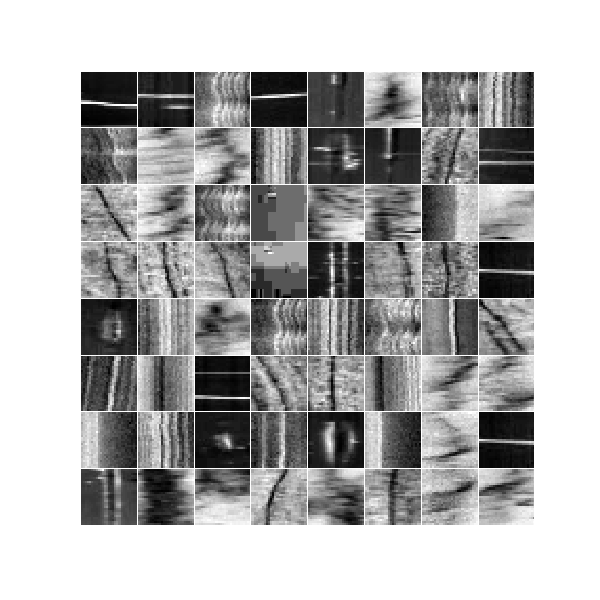
\includegraphics[width=0.9\linewidth]{figs/profile_examples.pdf}
	\caption{A collection of 64 by 64 image profiles taken from a hot steel rolling process.}
	\label{fig:Rolling}
\end{figure}

In literature, profile monitoring techniques can be categorized by their assumptions on the type of the functional relationship that they assume.
Linear profile monitoring can be considered the most basic profile monitoring technique, in which it is assumed that the profile can be represented by a  linear function. The idea is to extract the slope and the intercept from each profile and monitor its coefficients \parencite{zhu2009monitoring}. 
Regularization techniques can also be used in linear profile estimation. For example, Zou \etal utilize a multivariate linear regression model for profiles with the LASSO penalty and use the regression coefficients for Phase-II monitoring \parencite{zou2012lasso}.
However, the assumption of linear functional relationship can be quite limiting.
To address this challenge, nonlinear parametric models are proposed \parencite{Williams2007-ty,Jensen2009-tu,Noorossana2011-oj,Maleki2018-uo}.
These models assume an explicit family of parameterized functions and, their parameter estimations are estimated via nonlinear regression. In any cases, the drawback of all parametric models is that these models assume the parametric form is known beforehand, which might not always be the case.

% Literature: non-parametric Methods for certain types of profiles
Another large body of profile monitoring research focuses on the type of profile data where the basis of the representation is assumed to be known but the coefficients are unknown. 
For instance, to monitor smooth profiles, various non-parametric methods based on local kernel regression \parencite{zou2008monitoring,qiu2010nonparametric,zou2009nonparametric} and splines \parencite{chang2010statistical} are developed. 
To monitor the non-smooth wave-form signals, a wavelet-based mixed effect model is proposed
\parencite{paynabar2011characterization}. 
However, for all the aforementioned methods, it is assumed that the nonlinear variation pattern of the profile is well captured by a known basis or kernel.
Usually, there is no guidance on selecting the right basis of the representation for the original data and it normally requires many trial and error. 

%Here, we focus on the HD profiles where we cannot assume a parametric function form and the basis representation is unknown. 
In the case that the basis of HD profiles are not known, dimensionality reduction techniques are widely used. Principal component analysis (PCA) is arguably the most popular method in this context for profile data monitoring because of its simplicity, scalability, and good data compression capability. 
In \parencite{liu1995control}, PCA is proposed to reduce the dimensionality of the streaming data and, $T^{2}$ and $Q$ charts are constructed to monitor the extracted representations and residuals, respectively. 
To generalize PCA methods to monitor the complex correlation among the channels of multi-channel profiles, Paynabar \textit{et al} \parencite{paynabar2015change} propose a multivariate functional PCA method and apply change point detection methods on the function coefficients.
Along this line, tensor-based PCA methods are also proposed for multi-channel profiles, examples including uncorrelated multi-linear PCA \parencite{paynabar2013monitoring} and multi-linear PCA \parencite{grasso2014profile}. 
Finally, various tensor-based PCA methods \parencite{yan2015image} are compared and different test statistics are developed for tensor-based process monitoring.

The main limitation of all the aforementioned PCA-related methods is that the expressive power of linear transformations is very limited. Furthermore, each principal component represents a global variation pattern of the original profiles, which is not efficient at capturing the local spatial correlation within a single profile. Therefore, PCA requires a much larger latent space dimensions than the dimension of the actual latent space, yielding a sub-optimal and overfitting-prone representation. This phenomena hinders the profile monitoring performance. 

A systematic discussion of this issue is articulated in \parencite{Shi2016-tg}. 
In that work, the authors identify the problems associated with assuming a closeness relationship in the subspace that is characterized by Euclidean metrics.
They successfully observe that the intra-sample variation in complex high-dimensional corpora may lie on a nonlinear manifold as opposed to a linear manifold which is assumed by PCA and related methods. However, the authors only focus on applying manifold learning for Phase-I analysis, while Phase-II monitoring procedure is not touched upon \parencite{Shi2016-tg}.

Deep dimensionality reduction models have been proposed as an alternative to classical dimensionality reduction techniques in a handful.
Deep autoencoders have been proposed for profile monitoring for Phase-I analysis in \parencite{Howard2018-op}. 
Yan \etal \parencite{Yan2016-wa} compared the performance of contractive autoencoders and denoising autoencoders for Phase-II monitoring. 
Zhang \etal \parencite{Zhang2018-js} proposed a denoising autoencoder for process monitoring.
Aside from deterministic deep neural networks, only three works \parencite{wang2019systematic,Zhang2019-lu,lee2019process} proposed to use deep probabilistic latent variable models, specifically, variational autoencoders (VAE) \parencite{Kingma2013-dl}.
While they all show impressive results in terms of improvement over classical methods such as PCA, their empirical results are constrained to low-dimensional problems.
Some of the test statistics proposed in those works require a large number of Monte Carlo sampling, which can be prohibitively expensive for industrial settings with high throughput and limited computing capabilities.
Also, issues of extrapolation to out-of-distribution samples and learning disentangled representations with deep neural network based methods are not mentioned and therefore not addressed.
These issues are critical to assess the behaviour of deep neural networks, and thus monitoring statistics based on them, when faced with out-of-control samples.


In this paper, our main objective is to fill this gap in order to provide a unifying understanding of how deep latent variable models  should be used for Phase-II high-dimensional profile monitoring based on both theoretical understanding and empiricial results.
Our contributions can be listed as follows:
\begin{itemize}
    \item We provide a detailed review and comparison of previously proposed monitoring statistics for general deep latent variable model \parencite{wang2019systematic,Zhang2019-lu,lee2019process} in \ref{sec:bckgrnd:critique}.
    \item We will then propose two new theoretically grounded monitoring statistics SPE and KLD for general probabilistic latent variable models in \ref{sec:proposed-statistic}. We showed theoretically that these monitoring statistics are analogous to $Q$ and $T^2$ for PCA methods. 
    \item We will then show that for general deep latent variable models, only SPE is needed, where KLD is not recommended. We will show why this is the case from both theoretical understanding as well as performance evaluation. 
 % This proposed monitoring statistics takes into the consideration of the assumptions of the model, various sources of disturbances to the system, computational restrictions and behavioural issues peculiar to deep latent variable models.
    \item We carry out a simulation study carefully curated to demonstrate the peculiarities associated with deep latent variable models and demonstrate how the monitoring statistic we propose handle them in \ref{sec:simstudy}
    \item We support our results with a real-life case study on image profiles taken from a hot steel rolling process in \ref{sec:case-study}.
\end{itemize}

\section{Background}
\label{sec:bckgrnd}
In this section, we introduce some core concepts that are essential to comprehension of the methodology proposed in this study.
\subsection{Deep Learning}
\label{sec:bckgrnd:deep-learning}
Deep learning has enjoyed a tremendous resurgence in the last decade due to their superior performance that was unprecedented for many tasks such as image classification \parencite{krizhevsky2012imagenet}, machine translation \parencite{bahdanau2014neural}, 
and speech recognition \parencite{amodei2016deep}. In theory, under sufficient conditions, a two layer multilayer perceptron can approximate any function on a bounded region \parencite{cybenko1989approximation,Hornik1991-li}. Growing the width of shallow networks in an exponential fashion for arbitrarily complex tasks is not practical. It has been shown that deeper representations can often achieve the better expressive power than shallow networks with less parameters due to the efficient reuse of the previous layers  \parencite{eldan2016power}.


\subsection{Latent Variable Models}
\label{sec:bckgrnd:lvms}
Latent variables are powerful tools to model complex distributions over high-dimensional spaces.
The underlying assumption is that there exists a low-dimensional latent structure that explains well the variations in the high-dimensional observed space. Typically,  the density over observed variables can be decoupled into the distribution on the latent variables and the conditional distribution of observed variables given latent variables can be assigned as tractable families of distributions, which will be much more efficient than modeling the data distribution directly. 

A typical example of latent variable models is when the joint distribution is Gaussian factorized as in \ref{eq:gaussian-factorized}.
\begin{equation}
\label{eq:gaussian-factorized}
\begin{split}
\pz &= \Norm(\mbz;0,\mbI_{r})\\
\decoding &= \Norm(\mbx; \mu_{\mbtheta}(\mbz),\sigma^2 \mbI_{d}) \\
p_{\mbtheta}(\mbx,\mbz) &= \decoding\pz
\end{split}
\end{equation}
In the above formulation $\mbx \in \R^{d}$ are observed samples, $\mbz \in \R^{r}$ are latent variables while $\mu_{\mbtheta}\colon\R^{r}\to\R^{d} $ is a function paramterized by $\mbtheta \in \Theta$, that describes the relationship between the latent variables and the mean of the conditional. The Gaussian prior $\pz$ is typically chosen to be standard to avoid degenerate solutions \parencite[p. 307]{roweis1999unifying} and conditional covariance is typically assumed to be isotropic $\sigma^2 I_{d}$ to avoid ill-defined problems.
The aim is to approximate the true density $p_{\mbtheta}(\mbx) \approx p(\mbx)$ and this approximation can be obtained through marginalization:
$$
p_{\mbtheta}(\mbx) = \int p_{\mbtheta}(\mbx,\mbz) d\mbz
$$
Finally, in literature, there has been discussions about  whether the independent latent structure assumption $\pz = \Norm(\mbz;0,\mbI_{r})$ can lead to the discovery of the true disentangled variations, a task also known as disentangled representation learning \parencite[Sec. 3.5]{bengio2013representation}. Disentangled representations are useful to represent variations in latent variations due to its ability to separate out the independent factors. We are interested in whether and if so, how, such representations will be critical for profile monitoring. 

A famous member of the family of models described above is the probabilistic principal component analysis (PPCA) \parencite{tipping1999probabilistic}.
The parameters are optimized via a maximum likelihood estimation framework and it can be solved analytically due to the fact that $\mu_{\mbtheta}$ is a simple linear transformation enabling the optimization to reuse results from original solutions to the PCA problem.

\subsection{Deep Latent Variable Models}
The assumption of PPCA that the latent and observed variables have a strictly linear relationship can be quite restricting.
In real-world processes, it is likely that this relationship is highly nonlinear.
Deep latent variable models are a marriage of deep neural networks and latent variable models that aim to solve this problem.
We present two foundational members of this model family: Variational Autoencoders (VAE) \parencite{Kingma2013-dl} and Adversarial Autoencoders (AAE) \parencite{Makhzani2015-ei}.
We will refer to both of them as deep latent variable models (DLVMs) for short in the rest of the paper.

The main difference between PPCA and DLVMs is that the latter replace the linear transformation with a high-capacity deep neural network (called \textit{generative} or \textit{decoder}).
This is powerful in the sense that along with a general purpose prior $\pz$ a wide variety of densities can be modeled \parencite{kingma2019introduction}.
Unlike PPCA, these models will not have analytical solutions due to the complex nature of the neural network used.
Like most other deep learning models, their parameters have to be optimized via gradient descent for maximum likelihood.
The problem becomes even harder given the observation that the posterior $\decoding$ takes meaningful values only for a small sub-region within $\R^{r}$.
This makes sampling from the prior $\pz$ to estimate the likelihood prohibitively expensive.
Both models work around this problem using the importance sampling framework \parencite[p. 532]{bishop2006pattern}, where they introduce another network (called \textit{recognition} or \textit{encoder}) to approximate a proposal distribution $\encoding$ ---parametrized by $\mbphi$--- which will hopefully sample latent variables from a much smaller region that is more likely to produce higher posterior densities for a given input $\mbx$. 

The ultimate output of a trained DLVM is the likelihood estimator.
Once the two networks are trained, the log-likelihood $\log \ptheta(\mbx)$ can be approximated by a Monte Carlo sampling procedure with $L$ iterations \parencite[p. 30]{kingma2019introduction}:
\begin{equation}
\label{eqn:SummationLL}
\log \ptheta(\mbx) \approx \log \frac{1}{L} \sum_{l=1}^{L}\frac{\ptheta(\mbx,\mbz^{(l)})}{\qphizgivenx{\mbz^{(l)}}{\mbx}}    
\end{equation}

VAEs are trained to optimize the so-called evidence lower bound (ELBO), which is deemed a proxy to the likelihood:
\begin{equation}
\label{eqn:VAELoss}
\begin{split}
    \text{ELBO} &\triangleq \log\left( p(\mbx) \right) - \KL{\encoding}{q^{*}(\mbz|\mbx)} \\ 
	&= \E_{\mbz \sim q_{\mbtheta}} \log \decoding + \KL{\encoding}{p(\mbz)}
\end{split}
\end{equation}
where $\KL{\cdot}{\cdot}$ denotes the Kullback-Leibler divergence (KLD) between two distributions. 
The left-hand side is the quantity of interest while the right-hand side is the tractable expression that guides the updating of parameters $\mbtheta, \mbphi$ in an end-to-end fashion.

AAE (Gaussian posterior variant) \parencite{Makhzani2015-ei} uses a slightly different approach to impose the prior $\pz$ by replacing the KLD loss with adversarial training. 
In addition to finding good posterior proposals, recognition model $\encoding$ now has to convince a third neural network ---the discriminator network $D$--- that its samples are coming from standard Gaussian distribution.
The discriminator network also evolves through this process, getting better and better at discriminating non-standard samples and forcing the recognition model to improve itself further.
Formally, the discriminator tries to maximize the objective function given as follows:
\begin{equation}
\label{eqn:discloss}
	 L_{D} \triangleq  \E_{\pz} \log(1 - D(\mbz)) +  \E_{\encoding} \log(D(\mbz))
\end{equation}
This interplay of fooling-discriminating scheme results in a minimax game formalized as follows:
\begin{equation}
\label{eqn:aae-loss}
	\min_{\theta,\phi}\max_{D} \E_{z \sim \encoding}\log\decoding + L_{D}
\end{equation}
All three networks are trained concurrently to achieve a Nash equilibrium.

\subsection{Convolutional Layers}
Introduced in \parencite{lecun1989backpropagation}, convolutional layers have enabled tremendous performance increase in certain neural network applications where the data is of a certain spatial neighborhood structure such as images or audio waveform.
They exploit an important observation of such data, where the learner should be equivariant to translations.
This is an important injection of inductive bias into the network that largely reduce the number of parameters compared to the fully connected network by the use of parameter sharing. It eventually increase the statistical learning efficiency, especially for small samples.
It must be noted however, convolutional layers are not equivariant to scale and rotation as they are to translation.

\subsection{Review of $\Tsq $ and $Q$ statistics in PCA}
\label{sec:bckgrnd:ReviewPCA}
Process monitoring via PCA is typically undertook using the so-called $ \Tsq $ and $ Q $ statistics \parencite{Chen2004-px}. 
The $ Q $ statistic for PCA is defined as the reconstruction error between the real sample $ \mbx $ and the reconstructed sample $ \tilde{\mbx} $. Its geometric representation is how far the sample is away from the learned subpsace of in-control (IC) samples.  $ \Tsq $ represents how far the sample is away from the cluster of latent codes of the IC samples. 

The $ \Tsq $ statistics and $ Q $ statistic for PCA are defined as follows:
%TODO: give numbers to each line or not?
% No need
\begin{equation}
\begin{split}
	Q(\mbx) &= \gg \mbx - \tilde{\mbx} \gg^2 \\
	\Tsq_{PCA}(\mbx) &= \mbz^\top \mbSigma\inv_{r} \mbz = \mbx^\top \mbW_{r} \mbSigma\inv_{r} \mbW^\top_{r} \mbx,
\end{split}
\label{eqn: QTPCA}
\end{equation}
where matrix $ \mbW_{r} $ is the loading matrix, and $ \mbSigma\inv_{r} $ is the inverse of the covariance matrix when only the first $r$ principal components are kept. 
There are various methods to choose $r$ such as fixing the percentage of variation explained \parencite[p. 41]{Chiang2001-nu}.

For processes with relatively small latent and residual dimensionality, the upper control limits of these statistics for the $\alpha$\% Type-1 error tolerance is constructed by employing the normality assumptions of PPCA \parencite[p. 43-44]{Chiang2001-nu}.
However, using such measures for high-dimensional nonlinear profiles is prohibitively error-prone as both $r$ and $d$ will be much higher than the assumptions on chi-square distribution can tolerate.
As an alternative, non-parameteric methods to estimate upper percentiles are increasingly used for this purpose, such as simple sample percentile on a held-out set or fitting kernel density estimation to in-control statistics.

\subsection{Review and Critique of Previously Proposed Monitoring Statistics Proposed for VAE}
\label{sec:bckgrnd:critique}
Three works have considered VAE for process monitoring \parencite{wang2019systematic, Zhang2019-lu, lee2019process}, all of which propose different statistic formulations for monitoring.
Zhang \etal \parencite{Zhang2019-lu} formulate what they call $H^2$ which is basically the Mahalanobis distance of the mean of the proposal distribution from standard Gaussian distribution.
\begin{equation}
    H^2 = \mu_{\mbphi}(\mbx)^{\top}\mu_{\mbphi}(\mbx)
\end{equation}
The major drawback of using only this statistic is that it completely ignores the disturbances in residual distribution.

Lee \etal \parencite{lee2019process} claim to extend $T^2$ and $SPE$ of PCA for VAE.
For a given input $\mbx$ and a singe sample drawn from proposal $\mbz^{(l)} \sim \encoding$ and a reconstruction based on that sample $\mbx^{(l)} \sim p_{\mbtheta}(\mbx \g \mbz^{(l)})$, the proposed test statistics in this work are as follows:
\begin{equation}
\begin{aligned}
    T^{2} &= (\mbz^{(l)} - \bar{\mbz})^{\top}S_{\mbz}\inv(\mbz^{(l)} - \bar{\mbz}) \\
    SPE &= \gg \mbx^{(l)} - \mbx \gg_{2}^{2},
\end{aligned}
\end{equation}
where $\bar{\mbz}$ and $S_{\mbz}\inv$ are estimated over a single loop from the data. It is unclear why they would use such an extra step since for a well trained VAE, $\bar{\mbz}$ and $S_{\mbz}\inv$ would be approximately equal to the mean and covariance of the standard Gaussian distribution.
Instead, they take on the additional risk associated with the estimation.
The proposed control charting methodology suggests that these two statistics work in combination and at least one vote of either statistics is enough to make a detection.
The authors do not mention how false alarm rate can be fixed given this methodology.

Finally, Wang \etal propose the $R$ and $D$ statistics by focusing on the two major components of the tractable part of the objective function of VAE shown as in \ref{eqn:VAELoss}.
The $D$ statistic is simply the KL divergence between the prior and proposal.
For $R$ statistic, like \parencite{lee2019process}, they employ summary statistics over samples from proposal but also claim that sampling size can be fixed to one:
\begin{equation}
\begin{aligned}
    D &= \KL{\encoding}{p(\mbz)} \\
    R &= \frac{1}{L} \sum_{l=1}^{L} -\log q_{\mbtheta}(\mbx \g \mbz^{(l)}),
\end{aligned}
\label{eq: DR}
\end{equation}
$SPE$ in and $R$ are essentially the same quantities up to a constant, which makes them identical in the context of monitoring statistic because the rankings for the same testing samples given the same model will be the same for both.
This is why we will use term $R$ for both and reserve the name $SPE$ for the statistic we propose in \ref{sec:methodology}.
\section{Methodology}
\label{sec:methodology}
\subsection{Proposed Monitoring Statistic for Deep Latent Variable Models}
\label{sec:proposed-statistic}


Log-likelihood, $\log \ptheta(\mbx)$, arises as a natural candidate for monitoring statistic in the context of DLVMs.
That is, given a well trained DLVM, in-control samples should have relatively higher log-likelihood than out-of-control samples.
However, the required number of Monte Carlo samples---$L$ in \ref{eqn:SummationLL}--- can be prohibitively large to get meaningful estimates of the likelihood \parencite{Kingma2013-dl}, which do not satisfy the real-time monitoring requirement for high throughput systems. To address this issue, ELBO defined in \ref{eqn:VAELoss} can be used for a reasonable approximation:

\begin{equation*}
    \E_{\mbz \sim q_{\mbtheta}} \log \decoding + \KL{\encoding}{p(\mbz)}
\end{equation*}

To understand the role of both terms in process monitoring, we revisit the assumptions of the model described in \ref{eq:gaussian-factorized}. Let us formally represent an out-of-control distribution as  $p_{\delta}(\mbx) \neq p(\mbx)$. Since $p(\mbx) = \int p(\mbx\g\mbz)p(\mbz) d\mbz$, we can observe two sources of out-of-control behaviours: disturbances in latent distribution $p_{\delta}(\mbz) \neq \pz$ and disturbances in observable distribution $p_{\delta}(\mbx \g \mbz) \neq p(\mbx \g \mbz)$. 
Note that various combinations of these two disturbances cover disturbances in the entire process. One can argue that $\E_{\mbz \sim q_{\mbtheta}} \log \decoding $ can detect the disturbances in the observable space $p_{\delta}(\mbx \g \mbz) \neq p(\mbx \g \mbz)$ and  $\KL{\encoding}{p(\mbz)}$ represents the change in the latent space $p_{\delta}(\mbz) \neq \pz$. 
We know that for processes that can be accurately modeled by PCA, both terms play an important role \parencite{kim2003process} for process monitoring. 
We argue that this holds true for PPCA too.
To prove this, we link the monitoring statistics of PCA (see \ref{sec:bckgrnd:ReviewPCA}) to PPCA using the ELBO framework.

\begin{prop}
\label{prop: T2Q} 
We know from the definition of PPCA \parencite{tipping1999probabilistic} that the prior, encoding and decoding functions are normally distributed as:
\begin{equation*}
\begin{split}
p(\mbz)& = \Norm(0,\mbI)\\
\decoding &= \Norm(\mbW\mbz,\sigma^2 \mbI)  
\label{eq: Gaussian}
\end{split}
\end{equation*}
In this case, from PPCA, the encoder also follows the normal distribution as $\encoding =\Norm(\mu(\mbx),\Sigma_z)$, where $\mu(\mbx) = \mbM^{-1} \mbW^\top \mbx$ and  $\Sigma_z = \sigma^2\mbM^{-1})$, where $\mbM = \mbW^\top \mbW + \sigma^2 \mbI$.
Then, the two monitoring statistics can be defined as: 
\begin{equation}
    \label{eqn:KL_PPCA}
	\KL{\encoding}{p(\mbz)} = \frac{1}{2} \gg \mu(\mbx) \gg^2 + C_1
\end{equation}
\begin{equation}
    \label{eqn:E_PPCA}
	\E_{\mbz \sim q_{\mbtheta}} \log \decoding \propto \gg\mbx-\mbW \mu(\mbx) \gg^{2} + C_2
\end{equation}
where $C_1$ and $C_2$ are constants that doesn't depend on $x$.
\end{prop}
The proof is given in \ref{sec:PoofOfPropTQ}. 
Note that the constants do not affect out-of-control decisions. 
Thus, the test statistics $\KL{\encoding}{p(\mbz)}$ is equivalent to the $T^{2}$ Statistics of PCA as defined in \ref{eqn: QTPCA}, and $\E_{\mbz \sim q_{\mbtheta}}$ is equivalent the $Q$ statistic.
Consequently, we can argue that both statistics will play an important role given the linearity assumption of PPCA is reasonable.

However, we claim that $\KL{\encoding}{p(\mbz)}$ will not be useful for process monitoring if the process has a much more complex web of interactions between latent and obserable variables, and DLVMs are used for modeling the density function.
There are two reasons this is the case.

First, for such complex processes, most of the change or disturbances should be expected on residual distribution. 
According to \parencite{severson2016perspectives} faults in complex real-life processes tend to alter the existing relationship between latent sources of variation and what is observed, as opposed to pushing to most extreme cases in the latent variational sources.

Second, the encoder $\encoding$ is likely to lack two important features: disentangled representations and extrapolation capabilities. 
Disentangled representations are required for process monitoring because of the assumption on $\pz$ that latent factors are independent.
Entangled representations will lead to entangled monitoring statistic values for $\KL{\encoding}{p(\mbz)}$, interfering with the logistics of control charting.
Locatello \etal proves in \parencite[Thm. 1]{locatello2018challenging} that without proper inductive biases injected into the model, it is impossible to find disentangled representations.
Unfortunately, injecting such inductive biases requires detailed anticipation of variations among in-control samples as well as specialzed neural network structures, both of which are extremely challenging tasks given industrial settings.
Our motivating example, hot steel rolling process exhibited in \ref{fig:Rolling} is a good example of why this is the case.

Moreover, even if the representations are disentangled, correct mappings of $\encoding$ may still not be obtained.
This is due to an important shortcoming of deep learning based models. 
Deep neural networks approximates well only at a bounded domain defined by where the training set (i.e., in-control samples) is densely sampled from and the behaviour of the function is often unpredictable outside that domain. 
In other words, it may not extrapolate well beyond the domain of training samples.
We refer interested readers to \ref{app:rosenbrock} where we replicated this phenomena on a toy example.
To see why this is a problem, first note that the encoder $\encoding$ will only be trained with profiles densely sampled from the bounded region of in-control samples, for which $\pz$ are high.
The behavior of the encoder is uncertain for profiles coming from dense regions of out-of-control latent structure $p_{\delta}(\mbz)\neq\pz$.
We expect increased false negatives should the model falsely map these profiles onto high density regions of $\pz$ but not $p_{\delta}(\mbz)$.

Unlike $\KL{\encoding}{p(\mbz)}$, extrapolation and disentanglement issues in $\encoding$ along with extrapolation issues in $\decoding$ help $\E_{\mbz \sim q_{\mbtheta}} \log \decoding$ detect faults better, even when the disturbance is purely on latent structure.
Incorrect mappings by $\encoding$ will lead to incorrect generations by $\decoding$ and thus larger $\E_{\mbz \sim q_{\mbtheta}} \log \decoding$.
Second, even if the mapping was correct, we might have extrapolation issues in the decoder $\decoding$ which is another possibility for this statistic to capture disturbances in latent variations.
To see why this is the case, note that the encoder $\encoding$ is optimized to produce samples more from where $\pz$ is large. 
In turn, the decoder $\decoding$ will mostly be trained on samples from where $p_{\delta}(\mbz)$ is low. 
For disturbances in observable region $p_{\delta}(\mbx\g\mbz) \neq p(\mbx\g\mbz)$, it is trivial to see how $\E_{\mbz \sim q_{\mbtheta}} \log \decoding$ will be effective at capturing faults.

As of now, we have enough reasons to recommend the use of $\E_{\mbz \sim q_{\mbtheta}} \log \decoding$ as the only test statistic for a profile monitoring application that uses DLVMs.
This statistic is very similar to $SPE$ of \parencite{lee2019process} and $R$ \parencite{wang2019systematic}.
However, they both use random samples from the proposal distribution to estimate the expectation.
This approach may require a large number of samples to be generated and thus a large number of forward passes on a neural network, which is prohibitevely expensive in terms of computation.
We formulate a smarter way to approximate the test statistic, by using first order Taylor expansion for the moment of the log-likelihood.
We call this approximation $\oursacronym$, which is our final proposed statistic.

\begin{align}
    \label{eqn:propstat:final}
    \oursacronym &\triangleq \E_{\mbz \sim q_{\mbtheta}} \log \decoding \\
    &= \E_{\mbz \sim p_{\mbtheta}} \left[ \log q_{\mbtheta}(\mbx \g \mbz - (\mu_{\mbphi} - \mbz)) \right] \\
    &\approx \log\ptheta(\mbx \g \mu_{\mbphi}(\mbx)) \\ 
    &\propto \gg \mbx - \mu_{\mbtheta}(\mu_{\mbphi}(\mbx)) \gg_2^{2} + C_{3}
\end{align}
Again, the constant $C_3$ can be ignored given control charting logistics. Given a trained DLVM such as VAE or AAE, this quantity can be computed by forward passing the new profile from the process $\mbx$ through $\mu_{\mbphi}$ and $f_{\mbtheta}$ successively and calculating the squared prediction error, without any reparametrization.

\subsection{Profile Monitoring Procedure}
\label{sec:methodology:procedure}
A typical profile monitoring follows two phases: Phase-I analysis, and Phase-II analysis. Phase-I analysis focuses  on understanding the process variability by training an appropriate in-control mode, and selecting an appropriate control limit. 
Specifically when DLVMs are used, Phase-I analysis results in a trained model (i.e. an encoder and a decoder) and an Upper Control Limit (UCL) to help setup the control chart for each of the monitoring statistics.
In Phase-II, the system is exposed to new profile generated by the process to decide whether these profiles are in-control or out-of-control (OC).
Our experimentation plan, outlined below, is formulated to emulate this scenario to effectively assess the performance of any combination of a model, a test statistic and a disturbance scenario.
\begin{itemize}
	\item Obtain IC dataset $ \dataset $ and partition it into train, validation and test sets $ \dataset^{trn} $,$ \dataset^{val} $,$ \dataset^{tst} $
	\item Train the DLVM using samples from $\dataset^{trn}$ over a pre-defined grid of hyperparameters.
	\item Choose the trained DLVM with the lowest reconstruction error over $\dataset^{val}$ and proceed with that.
	\item Calculate test statistic for all $ \mbx \in \dataset^{val} $ and take it's \nth{95} percentile as the UCL.
	\item Record the estimated false alarm rate (FAR)  as the average number of samples $ x \in \dataset^{tst} $ that are misclassified as OC because their test statistic yields a number higher than UCL.
	\item Start admitting profiles from the disturbed process. Calculate test statistic using the trained DLVM. If test statistic is over UCL, identify the sample as OC.
\end{itemize}
For each DLVM type, we train 10 different model instances with different seeds to account for inherent randomness due to weight initialization of DLVMs.

\subsection{Model Architectures \& Implementation Details}
 
Both VAE and AAE use the same encoder-decoder structure outlined in \ref{tab:model-architectures}.
The layers used that builds the model architectures used in this study are summarized as follows:
 
\begin{itemize}
	\item C($O, K, S, P$): Convolutional layer with arguments referring to number of output channels $O$, kernel size $K$, stride $S$ and size of zero-padding $P$.
	\item CT($O, K, S, P$): Convolutional transpose layer with arguments referring to the number of output channels $O$, kernel size $K$, stride $S$, and size of zero-padding $P$.
	\item FC(I, O): Fully connected layer with arguments referring to input dimension $I$ and output dimension $O$.
	\item A: Activation function. Can either be Rectified linear unit (ReLU) or Leaky ReLU with a negative slope $0.2$.
	\item S(): Sigmoid activation.
\end{itemize}
Here, C(), CT(), and FC() are considered the linear transformation layers while R(), LR(), and S() are considered the nonlinear activation layers. 
Strided convolutions can be used to decrease the spatial dimensions in the encoders. 
Pooling layers are typically not recommended in autoencoder-like architectures \parencite{radford2015unsupervised}. 
Convolutional transpose layers are used to upscale latent codes back to observable dimensions. 
Leaky ReLU has been suggested to improve performance in adversarial training \parencite{salimans2016improved} but we include that option for both VAE and AAE for fairness.

The sequential order of the computational graphs used for this study are summarized in \ref{tab:model-architectures}. 
For AAE and VAE, an encoder will output $2r$ nodes which is a concatenation of the inferred posterior mean and variance, both are of length $r$. 
For AAE, a simple multilayer perceptron---the discriminator---is created additionally.  
A grid of hyperparameters are considered for learning rate, batch size, and the number of latent dimensions $r$.

\begin{table}[!t]
	\renewcommand{\arraystretch}{1.3}
	\caption{Architecture details of deep neural networks used in this study}
	\label{tab:model-architectures}
	
	\begin{tabular}{ll}
		\toprule
		Module & Architecture \\
		\midrule
		Encoder & C(32, 4, 2, 1) - A - C(32, 4, 2, 1) - A - C(64, 4, 2, 1) - A - C(64, 4, 2, 1) - A - C(64, 4, 1, 0) - FC(256, $2r$) \\
		Decoder & FC($r$, 256) - A - CT(64, 4, 0, 0) - A - CT(64, 4, 2, 1) - A - C(32, 4, 2, 1) - CT(32, 4, 2, 1) - A - CT(1, 4, 2, 1) \\ 
		Discriminator & FC($r$, 512) - FC(512, 256) - FC(256, 1) - S() \\
		\bottomrule
	\end{tabular}
\end{table}

\section{Simulation Study Analysis and Results}
\subsection{Simulation Setup}\label{sec:simsetting}
We first evaluate the performance of the deep latent variable models in a simulation setting inspired by the work of Shi \etal \parencite{Shi2016-tg}. The simulation procedure produces 2D point clouds that resemble the scanned topology of a gasket bead.
Let each point on a $64$ by $64$ grid be denoted by a tuple $\mbp = (p_0, p_1)$.
The values of the tuples stretch from $0$ to $1$ equally spaced, left to right and bottom-up.
Each tuple takes a value based on its location through a function $\mbp \mapsto f(\mbp; \czero, r) + \epsilon$, where $\epsilon \sim \Norm(0, 1\times10^{-2})$ is i.i.d Gaussian noise.
The function $f$ is parametrized by the horizontal center location  of the bead $ \czero $, and the radius of the bead $r$.
The vertical center of the bead is fixed to be at the center.
Given any parameter set $\{c_0,r\}$, each pixel $\mbp$ can be evaluated with the following logic:
\begin{equation}
\label{eq:gasketfun}
\begin{split}
g(\mbp; c_0,r)&=1-\frac{(p_0 - \czero)}{r}^2 - \frac{(p_1 - 0.5)}{r}^2 \\
	f(\mbp; c_0,r)&= 
	 \begin{cases} 
	 \sqrt{g(\mbp; c_0,r)} &\mbox{if } g(\mbp; c_0,r) \geq 0 \\ 
 0 & \mbox{if } g(\mbp; c_0,r)<0 
	\end{cases}
\end{split}
\end{equation}

The samples are best visualized as grayscale images as shown in \ref{fig:gasketgrid}.
\begin{figure}[!t]
    
    \label{fig:gasketgrid}
    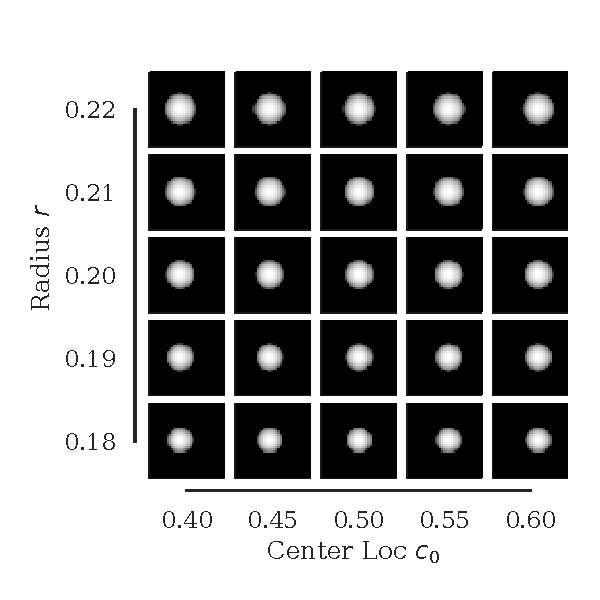
\includegraphics[width=0.9\linewidth]{figs/gasket.pdf}
    \caption{Gasket profiles depicted as grayscale images simulated with radius and center location they coincide with on the axes.}
\end{figure}


We define the sources of variation in IC gasket beads by two latent variables sampling from independent Gaussian distributions:
\begin{equation}
\begin{split}
	\czero \sim \Norm(0.5, 1\times10^{-2}) \\
	r \sim \Norm(0.2, 6.25\times10^{-4})
	\end{split}
\end{equation}

Finally, we will consider the following four types of OC variation patterns for the system. 
\begin{itemize}
	\item \textbf{Location shift.} the mean of the process that generates $ \czero $ is altered by an amount $ \delta $ as in $\czero \sim \Norm(0.5 + \delta\times10^{-2}, 1\times10^{-2})$.
	\item \textbf{Width shift.} the mean of the process that generates $ a $ is perturbed by an amount $ \delta $ as in $r \sim \Norm(0.2+\delta\times10^{-4}, 6.25\times10^{-4})$. 
	\item \textbf{Mean shift.} all of the pixels are added an additive disturbance $ \delta $ as in $f(\mbp; c_0,r) \leftarrow f(\mbp; c_0,r) + \delta$.
	\item \textbf{Magnitude shift.} all of the pixels are added an multiplicative disturbance $ \delta $ as in $f(\mbp; c_0,r) \leftarrow f(\mbp; c_0,r) * \delta$
\end{itemize}
Here, $ \delta $ is the intensity of the change.
Note that location shift and width shift represent disturbances in residual distribution $p_{\delta}(\mbx \g \mbz)$.
An important distinction between the two is that location equivariance is injected into convolutional networks but not scale equivariance, therefore we expect different reactions to these changes by deep convolutional latent variable models in terms of disentanglement.
The other two cases, mean shift and magnitude shift, represent disturbances in latent prior $p_{\delta}(\mbz)$.
The training, validation, and testing IC or OC samples are generated of size 500 each. 

\subsection{On the disentanglement and extrapolation performance of the recognition network $\encoding$}
\label{sec:simstudy:recognition}
To investigate the disentanglement and extrapolation performance of the recognition network we employ the following procedure. 
First, we train a DLVM (in this case a VAE with latent code being 2-dimensional) to convergence using in-control samples as described in \ref{sec:simsetting}. 
Then, we feed intentionally picked examples on the space of our latent variables ---radius $r$ and center location $\czero$--- into the recognition network to obtain their respective proposal distributions.
The points are picked inside and outside the tolerance region of the two quality characteristics to be compared against their mapping onto the representation space.
Finally, we sample 150 points from the proposals and plot them on the representation space.
The results are shown in \ref{fig:proposals}, where the samples from the proposal can be traced back to the true sources of variation. We observe an overall trend that distributions are not laid out in regards to the layout of the true sources of variation after they are mapped to the representation space. It shows that the disentanglement is not reconstructed via the VAE framework. 

Furthermore, we would like to study the anomaly detection performance. We observe that the extreme cases of the center location $\czero$ (i.e., Case 0, 3, 6, 2, 5, 8) are actually mapped outside or near the boundary of the circle. For the extreme cases of radius, only extremely large radii  (i.e., Case 7) result in extreme latent codes. This implies that circles with small radii will be missed by the monitoring statistics based purely on latent code (i.e., Case 1).

We only achieved partial disentanglement and that relates to the location only because we have translational equivariance in our convolutional architecture.
That demonstrates that our findings are in agreement with our rationale behind the proposed statistic outlined in \ref{sec:proposed-statistic}.
In other words, without extrapolation and disentanglement, we do not expect any monitoring statistic based purely on the output of the recognition network---such as $H^{2}$, $T^{2}$ or $D$ discussed in \ref{sec:bckgrnd:critique}--- to be robust enough to be safely employed in a process control mission.

The finding is also consistent with the one presented in \parencite[Thm. 1]{locatello2018challenging}.
Without proper inductive biases ---which is usually a very challenging task for industrial settings--- it is impossible for a latent variable model to learn disentangled representations. 

\begin{figure}[t]
    
    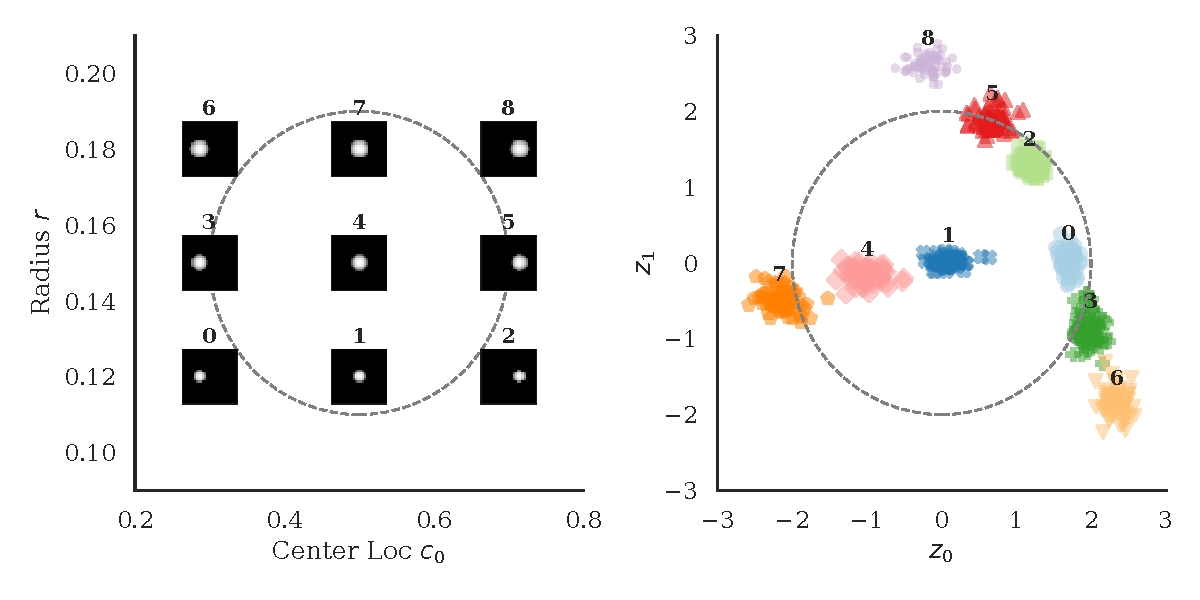
\includegraphics[width=\linewidth]{figs/proposals.pdf}
    \caption{Figure depicting the behaviour of the recongition network of a VAE trained with in-control gasket sampled. On the left nine gasket profiles whose latent variables are picked from in and out of the tolerable region of radius and center location. The tolerable region is represented by the gray dashed circle, a curve of isodistant points in terms of Mahalanobis distance to in control distribution. On the right, 150 latent codes sampled from each proposal (associated with the same id numbers on the top).  Isodistant curve for standard Gaussian that is probability-wise equivalent to the one on the left is depicted as a gray dashed circle.}
    \label{fig:proposals}
\end{figure}

\subsection{On the extrapolation performance of the generator network $\decoding$}
\label{sec:simstudy:generator}
\ref{fig:manifold_vae} depicts the extrapolation performance of the generator $\decoding$ of the same DLVM described in \ref{sec:simstudy:recognition} trained on in-control samples described in \ref{sec:simsetting}.
We observe two important behavior: the posterior gets distorted beyond two or three standard deviations and the representations are partially disentangled in line with the behaviour of its encoder depicted in \ref{fig:proposals}.
To reiterate, we observe that our generator cannot reason well beyond the bounds of its training samples.
We observe that variation comes to a halt beyond fifth standard deviation and roundness of beads becomes cluttered.
We observe a much severe case of the same for an example trained AAE as shown in \ref{fig:manifold_aae} where clutters start as early as second standard deviation.

It is straightforward to define disentanglement in the context of the simulation case since we have explicit control over the semantics and variations in the data.
Ideally, we want a DLVM with two-dimensional latent code to capture variations in radius and center location independently.
What we observe from both manifold figures is that variations in radius and location are convoluted.
The situation can be understood better when \ref{fig:manifold_vae} and \ref{fig:proposals} are jointly examined.
DLVMs, without specific inductive biases injected into the networks, will not discover the true latent variables and cannot extrapolate well beyond the training domain, which leaves the latent variables method not useful. 
 
We also want to make a remark that we tried the beta-VAE framework explained in \parencite{higgins2017beta} to remedy the problem but failed to get disentangled representations even for this simple case. The lack of training samples (i.e., 500 samples) may be another reason why the disentanglement is not clear.   

However, unlike the case for recognition network, the errors of generative network beyond the training region are indeed welcomed as they will inflate the negative log-likelihood.
Along with the findings \ref{sec:simstudy:recognition}, these findings support the rationale behind the statistic we propose in \ref{sec:proposed-statistic}.

\begin{figure}[!t]
    
    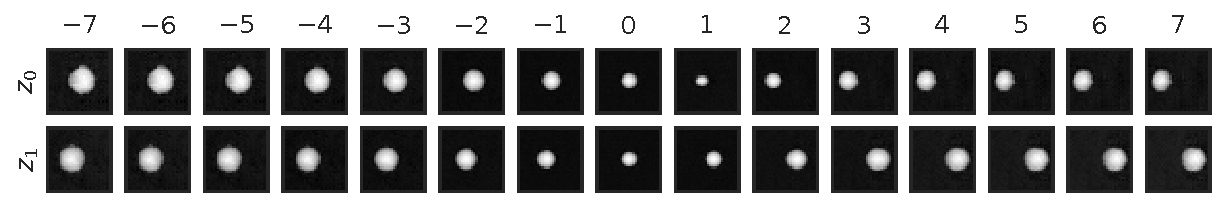
\includegraphics[width=0.9\linewidth]{figs/manifold_vae.pdf}
    \caption{Figure depicting per-dimension manifold of a VAE with two-dimensional latent code, trained on in-control gasket samples. Each row represents which latent dimension is altered while the other dimension is fixed at zero. Each column represents what value is assigned to that latent dimension that is represented by the row label.}
    \label{fig:manifold_vae}
\end{figure}


\begin{figure}[!t]
    
    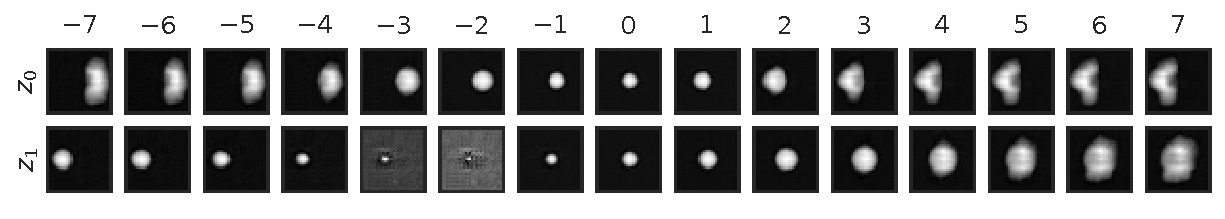
\includegraphics[width=0.9\linewidth]{figs/manifold_aae.pdf}
    \caption{Figure depicting per-dimension manifold of a AAE with two-dimensional latent code, trained on in-control gasket samples. Each row represents which latent dimension is altered while the other dimension is fixed at zero. Each column represents what value is assigned to that latent dimension that is represented by the row label.}
    \label{fig:manifold_aae}
\end{figure}

\subsection{Comparison of detection performance of proposed statistics}
\begin{figure}[!t]
    
    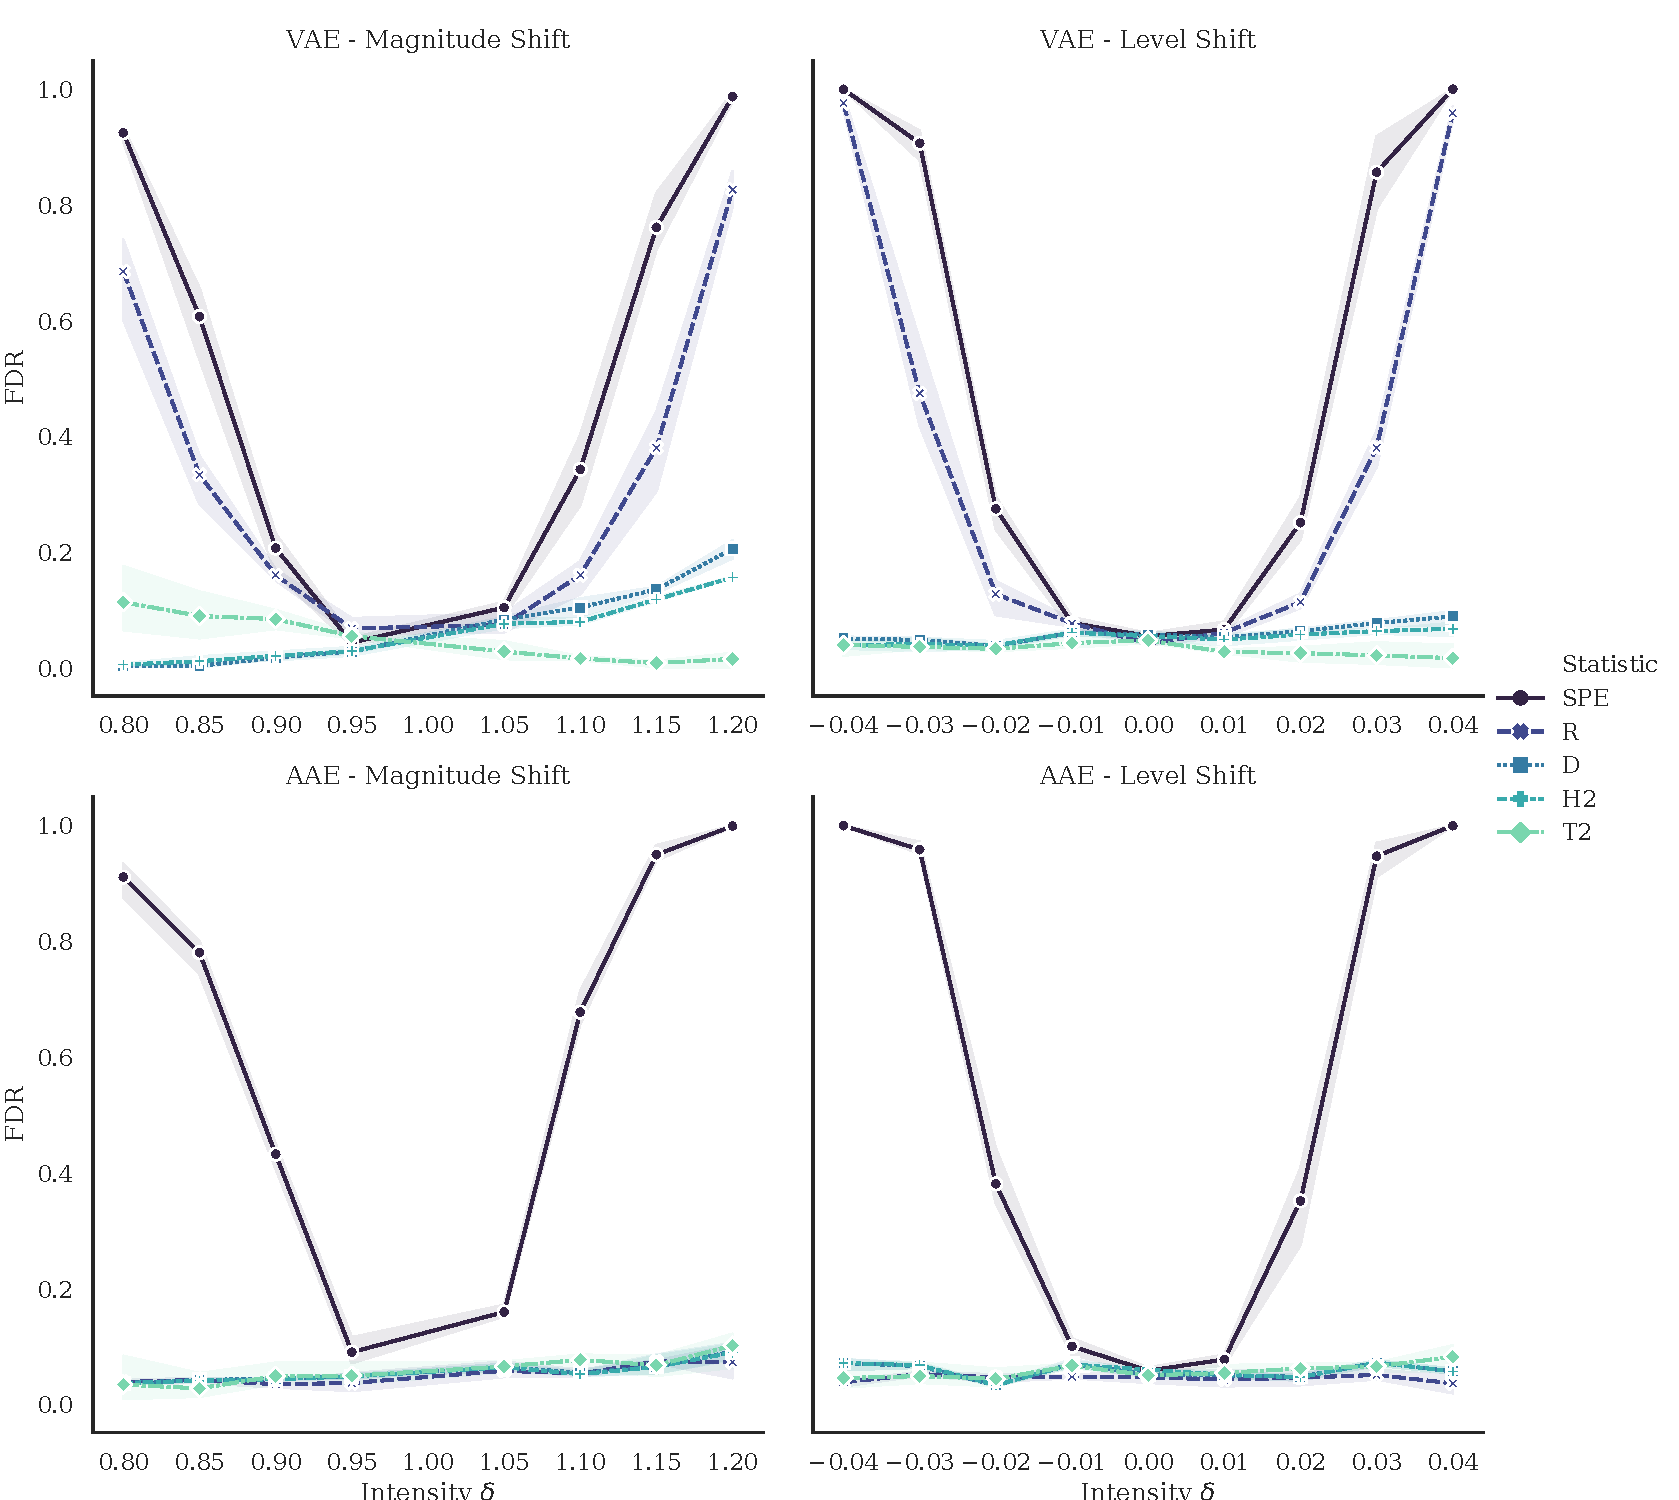
\includegraphics[width=\linewidth]{figs/disturbance_on_pxz.pdf}
    \caption{Fault detection rates (on the y-axis) for varying models (rows) and varying intensities (x-axis) of different disturbance types (columns) occuring on residual distributions. Bands represent 95\% confidence interval estimated around mean detection rates. 
    }
    \label{fig:disturbance_on_pxz}
\end{figure}
\begin{figure}[!t]
    
    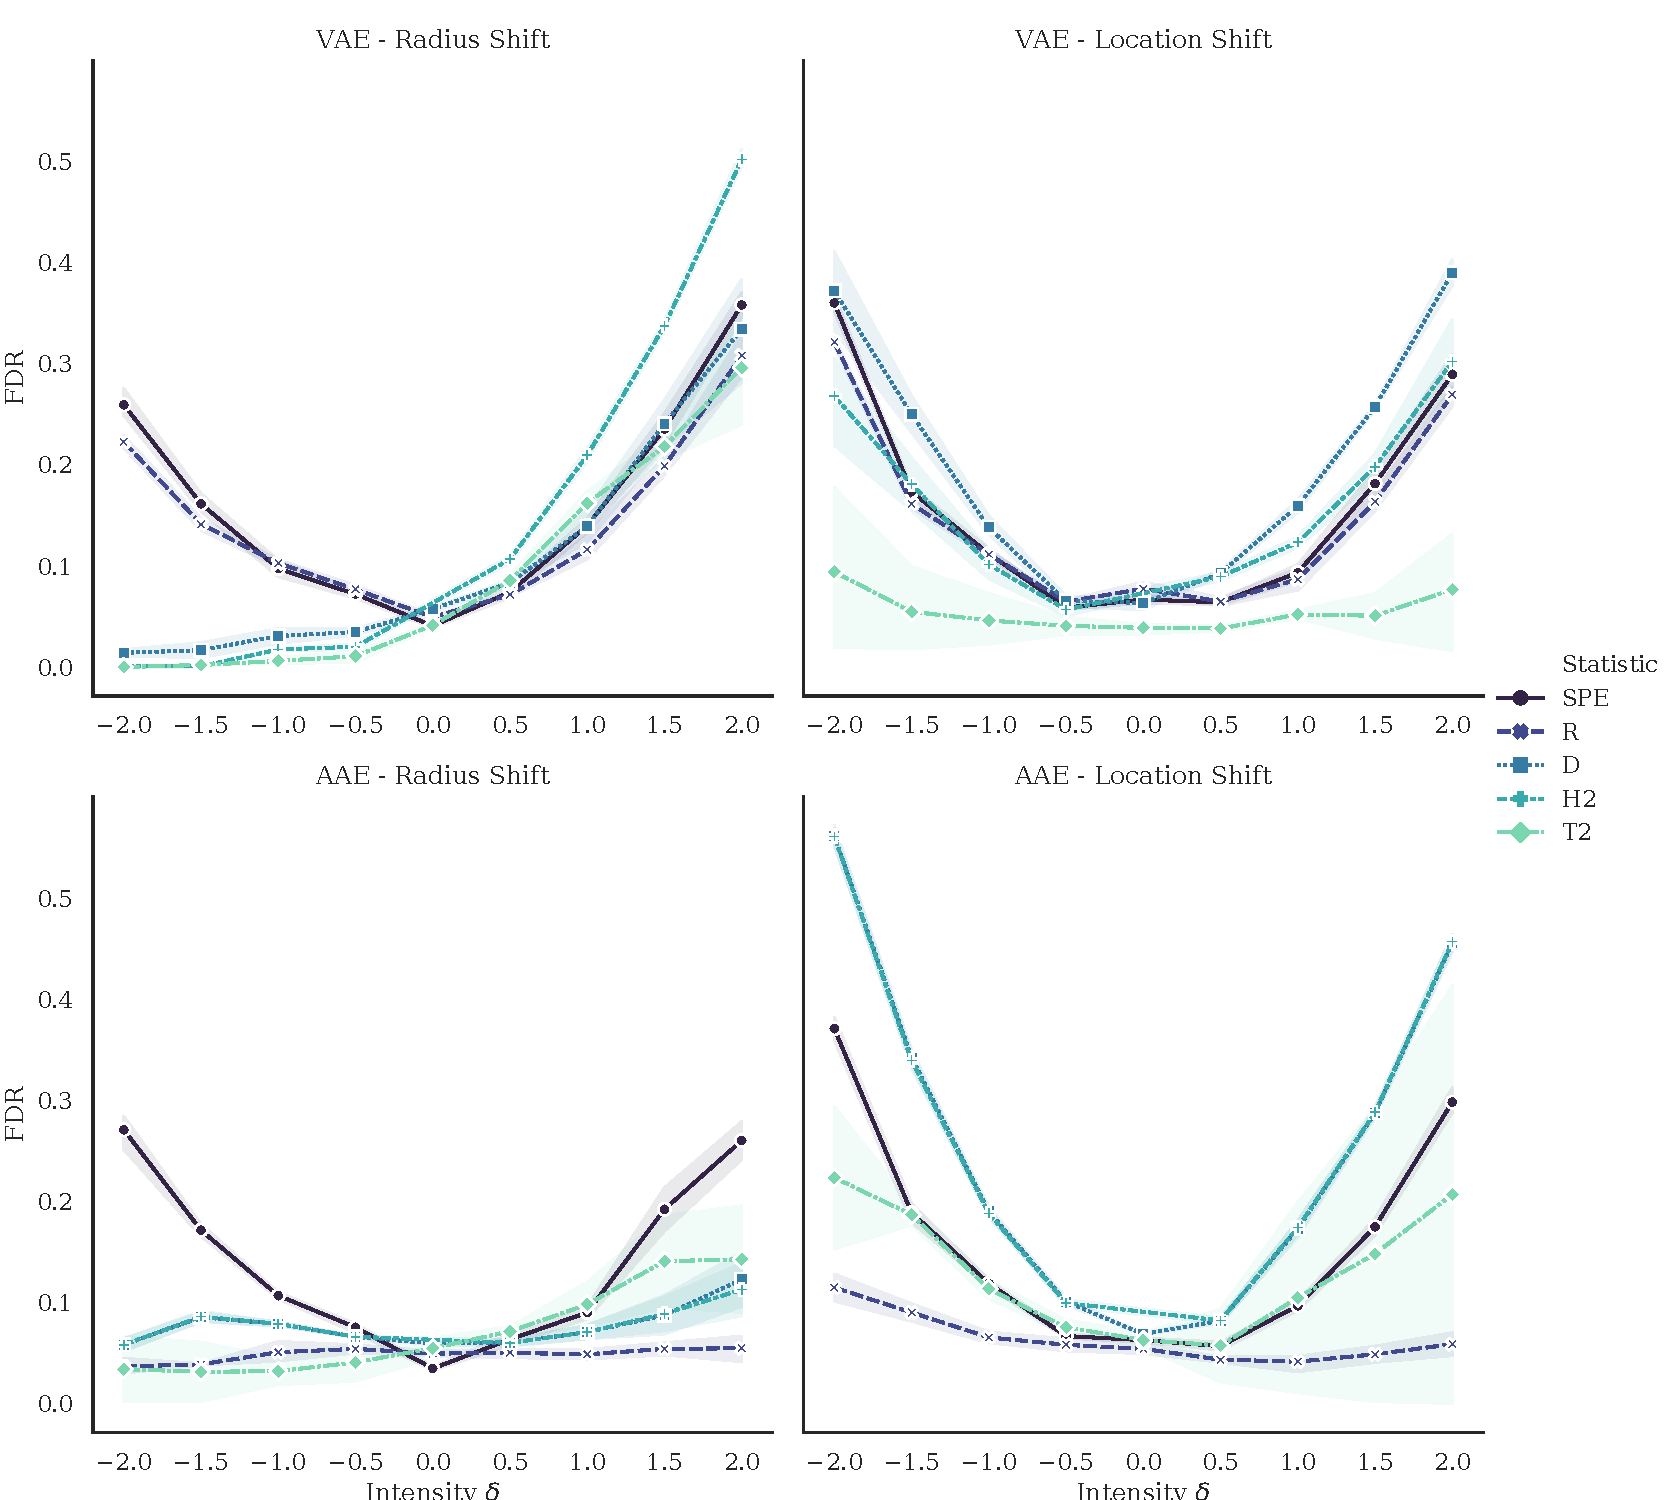
\includegraphics[width=\linewidth]{figs/disturbance_on_pz.pdf}
    \caption{Fault detection rates (on the y-axis) for varying models (rows) and varying intensities (x-axis) of different disturbance types (columns) occuring on latent distributions. Bands represent 95\% confidence interval estimated around mean detection rates.}
    \label{fig:disturbance_on_pz}
\end{figure}
We now compare the proposed statistics based on how accurately they detect profiles from out-of-control processes outlined in \ref{sec:simsetting}.
The first condition we must check is the robustness of the statistics by making sure all proposed statistics have roughly similar false alarm rate on the held-out in control test set, which should also be reasonably close to the desired rate 5\%.
\ref{tab:far} demonstrates that this is the case for all of them.

\begin{table}[t]
\renewcommand{\arraystretch}{1.3}
\caption{False alarm rates on held-out dataset averaged over 10 replications per model and monitoring statistic. Standard deviations are in parentheses.} 
\label{tab:far}

\begin{tabular}{lccccc}
\toprule
Statistic &              SPE &                R &                D &               H2 &               T2 \\
Model &                  &                  &                  &                  &                  \\
\midrule
AAE         &  0.031(0.001) &  0.045(0.009) &  0.043(0.001) &  0.043(0.001) &  0.058(0.007) \\
VAE         &  0.031(0.006) &  0.051(0.005) &  0.044(0.004) &  0.052(0.005) &  0.043(0.009) \\
\bottomrule
\end{tabular}
\end{table}

Through \ref{fig:disturbance_on_pxz}, we observe a clear superiority of $SPE$ over other methods when the disturbance is on the residual distribution.
It can be easily understood why $D$, $H^2$ and $T^2$ fail in this case, that they are purely computed using the proposal distribution $\encoding$.
The reason why $R$ underperforms than $SPE$ is more subtle. 
Given only a single sample from the proposal, $R$ becomes very sensitive to the estimation of variance while MAP estimation yields strong and robust performance across the board.
In our observations, AAE models yield much larger dispersion on proposals than VAE and this is why $R$ has performs even more poorly for AAE compared to VAE.
This is likely to be related to adversarial training.

For the latter two disturbances occurring purely on latent dimensions, results are presented in \ref{fig:disturbance_on_pz}.
We observe more mixed results where generally $SPE$, $D$ and $H^2$ tend to perform better than $R$ and $T^2$.
A commonality between the former three is that they don't rely on random samples, supporting argument against this practice.
One important observation to be made about $D$ and $H^2$ is that their detection performance do not always increase with increasing magnitude of intensities while this is not the case for $SPE$.
The reader is referred to the two left quadrants of \ref{fig:disturbance_on_pz} to observe this behavior.
This is due to the partial disentanglement (or entanglement) issue discussed in \ref{sec:simstudy:recognition} and just as expected, disturbances causing smaller radii are completely missed by $D$ and $H^2$.
However, $D$ and $H^2$ works well for a scenario that is extremely unlikely in real-life: that when the disturbance is purely on the latent space. Even then, $SPE$ still demonstrates decent performance regardless of the model and the direction of intensity of disturbance.
We think there is not enough evidence to justify deploying a latent code based statistic such as $D$ and $H^2$ considering the potential increase in false alarms.

In summary, this simulation study suggests that $SPE$ is the most reliable statistic among the statistics proposed for DLVMs so far.
In the next section, we test this hypothesis on a real life example using profiles from a hot steel rolling process.

\section{Case Study Analysis \& Results}
\label{sec:case-study}
% TODO (@DS): how many anomaly samples do we have?
% TODO (@DS): Add a figure to illustrate both normal and abnormal samples, with one image in each class

Our dataset consists of center-cropped image profiles from a hot-steel rolling process, which is shown in \ref{fig:Rolling}. 
There are 13 classes of surface types identified by the domain engineers.
Four of these classes---0,1,9 and 11--- are considered as in-control.
There are in total 338 images in these classes.
The other nine classes make up the out of control cases and they have in combination 3351 images to report detection accuracy for.
We randomly partition the IC corpus to fix train, validate and test sets with 60\%-20\%-20\% relative sizes respectively.
The rest of the procedure followed is outlined in \ref{sec:methodology:procedure}.
Same as in simulation study, to account for randomness in weight initialization, we replicate the experiment with 10 different seeds. 
The results are summarized in \ref{tab:rolling_results}.
They show strict similarity with the results in \ref{fig:disturbance_on_pxz}. 
$SPE$ dominates for each of the candidate DLVM and $R$ is the runner-up while statistics based on encoders suffer quite low and often none detection performance.

For completeness, we also include a comparison of our proposed statistic against the baseline method PCA where 90\% of the variance is retained.



To support our claim of ineffectiveness of the statistics based on the latent space such as $H^2$ statistics, we refer the reader to \ref{fig:T2vsQ}. \ref{fig:T2vsQ-a} shows the 2-D latent code of the AAE model given a set of OC samples. Since the 2-D latent code of OC samples are also close to the standard normal distribution, $H^2$ statistics will not be able to detect these OC behaviors. The ineffectiveness of $H^2$ statistics is validated in \ref{fig:T2vsQ-b}, where the density of $H^2$ distribution for OC and IC samples are largely overlapped. \ref{fig:T2vsQ-c} shows the reconstruction error of the images given the same 2-D latent code. From these images, it is clear that the reconstructed images are very different from the OC images, where $SPE$ can be used to capture such changes. The effectiveness of $SPE$ is also shown in \ref{fig:T2vsQ-d}, where the distributions of IC and OC samples do not have much overlap at all. 

\begin{table}[t]
\renewcommand{\arraystretch}{1.3}
\caption{Summary of fault detection accuracies on out-of-control cases averaged over 10 replications per model and monitoring statistic. Standard deviations are in parentheses. Bolded values represent the maximum within each model, across different statistics.}
\label{tab:rolling_results}

\begin{tabular}{lccccc|ccccc}
\toprule
Model & \multicolumn{5}{c}{AAE} & \multicolumn{5}{c}{VAE} \\
Statistic &         SPE &           R &           D &          H2 &          T2 &         SPE &           R &           D &          H2 &          T2 \\
Fault ID &             &             &             &             &             &             &             &             &             &             \\
\midrule
2                &  \textbf{0.33}(0.19) &  0.02(0.03) &  0.00(0.00) &  0.00(0.00) &  0.26(0.45) &  \textbf{0.44}(0.06) &  0.37(0.03) &  0.00(0.00) &  0.00(0.00) &  0.00(0.00) \\
3                &  \textbf{0.84}(0.02) &  0.21(0.08) &  0.00(0.00) &  0.00(0.00) &  0.21(0.13) &  \textbf{0.85}(0.01) &  0.84(0.01) &  0.17(0.06) &  0.23(0.04) &  0.03(0.03) \\
4                &  \textbf{0.61}(0.09) &  0.10(0.03) &  0.00(0.00) &  0.00(0.00) &  0.11(0.19) &  \textbf{0.75}(0.05) &  0.62(0.02) &  0.00(0.00) &  0.00(0.00) &  0.00(0.00) \\
5                &  \textbf{0.99}(0.00) &  0.12(0.09) &  0.81(0.01) &  0.83(0.02) &  0.04(0.07) &  \textbf{1.00}(0.00) &  \textbf{1.00}(0.00) &  0.58(0.07) &  0.62(0.09) &  0.00(0.00) \\
6                &  \textbf{0.73}(0.02) &  0.05(0.04) &  0.00(0.00) &  0.00(0.00) &  0.32(0.48) &  \textbf{0.80}(0.01) &  0.79(0.01) &  0.06(0.03) &  0.15(0.08) &  0.05(0.05) \\
7                &  \textbf{0.11}(0.00) &  0.04(0.01) &  0.00(0.00) &  0.00(0.00) &  0.00(0.00) &  \textbf{0.17}(0.01) &  0.13(0.01) &  0.01(0.01) &  0.01(0.01) &  0.00(0.00) \\
8                &  \textbf{0.51}(0.11) &  0.06(0.04) &  0.00(0.00) &  0.00(0.00) &  0.28(0.48) &  \textbf{0.70}(0.07) &  0.64(0.02) &  0.00(0.00) &  0.00(0.00) &  0.00(0.00) \\
10               &  \textbf{0.54}(0.03) &  0.07(0.02) &  0.00(0.00) &  0.00(0.00) &  0.05(0.09) &  \textbf{0.57}(0.05) &  0.49(0.03) &  0.00(0.00) &  0.00(0.00) &  0.00(0.00) \\
12               &  \textbf{0.82}(0.03) &  0.07(0.06) &  0.00(0.00) &  0.00(0.00) &  0.15(0.22) &  \textbf{0.80}(0.02) &  0.79(0.01) &  0.00(0.00) &  0.00(0.00) &  0.00(0.00) \\
13               &  \textbf{0.76}(0.01) &  0.05(0.03) &  0.00(0.00) &  0.00(0.00) &  0.09(0.16) &  \textbf{0.77}(0.02) &  0.71(0.04) &  0.00(0.00) &  0.00(0.00) &  0.01(0.00) \\
\bottomrule
\end{tabular}
\end{table}

\begin{table}[t]
    
    \caption{DLVM detection rate performance on hot steel rolling faulty cases compared against PCA with 90\% variance retained and $Q$ statistic is used. Best performers bolded on each row. Standard deviation over 10 replication is in 	.}
    \renewcommand{\arraystretch}{1.3}
    \begin{tabular}{lccc}
    \toprule
    Model &           PCA &      AAE &      VAE \\
    Fault ID &               &               &               \\
    \midrule
    2                &  0.00(0.00) &  0.33(0.19) &  \textbf{0.44}(0.06) \\
    3                &  0.78(0.00) &  0.84(0.02) &  \textbf{0.85}(0.01) \\
    4                &  0.56(0.00) &  0.61(0.09) &  \textbf{0.75}(0.05) \\
    5                &  0.99(0.00) &  0.99(0.00) &  \textbf{1.00}(0.00) \\
    6                &  0.52(0.00) &  0.73(0.02) &  \textbf{0.80}(0.01) \\
    7                &  0.11(0.00) &  0.11(0.00) &  \textbf{0.17}(0.01) \\
    8                &  0.34(0.00) &  0.51(0.11) &  \textbf{0.70}(0.07) \\
    10               &  0.29(0.00) &  0.54(0.03) &  \textbf{0.57}(0.05) \\
    12               &  0.69(0.00) &  \textbf{0.82}(0.03) &  0.80(0.02) \\
    13               &  0.56(0.00) &  0.76(0.01) &  \textbf{0.77}(0.02) \\
    \bottomrule
    \end{tabular}
    \label{tab:rolling:vsPCA}
\end{table}


\section{Conclusion}
\label{sec:conclusions}

\printbibliography



\appendix
\refalias{section}{appendix}
\section{Proof of Proposition \ref{prop: T2Q}}
\label{sec:PoofOfPropTQ}
Kullback-Leibler divergence between two multivariate Gaussian distributions has a closed form solution. 
If we define these distributions as $p_{0} = N(\mbz;\mbmu_{0}, \mbSigma_{0})$ and $p_{1} = N(\mbz;\mbmu_{1}, \mbSigma_{1})$ where $\mbmu$ and $\mbSigma$ are respective mean vectors and covariance matrices, then according to \parencite{hershey2007approximating} the closed form solution will be the following:
\begin{align*}
\KL{p_{0}}{p_{1}} & =\frac{1}{2}[\log\frac{\g\mbSigma_{1}\g}{\g\mbSigma_{0}\g}+Tr(\mbSigma_{1}\inv\mbSigma_{0})-r \\
 & +(\mu_{0}-\mu{1})^{\top}\mbSigma_{1}\inv(\mu_{0}-\mu{1}) ]
\end{align*}
Since $\encoding =\Norm(\mu(\mbx),\mbSigma_z)$ and $p(\mbz) = \Norm(0,\mbI)$, we can derive that 
\begin{align*}
\KL{\encoding}{p(\mbz)} &= \frac{1}{2}\left[ -\log\g\mbSigma_z\g + Tr(\mbSigma_z) -r \right] + \frac{1}{2} \mu(\mbx)^{\top}\mu(\mbx) \\
						&= \frac{1}{2} \mu(\mbx)^{\top}\mu(\mbx) + C,
\end{align*}
where $C = -\log\g\mbSigma_z\g + Tr(\mbSigma_z) -r $ is a constant, which doesn't depend on $\mbx$. 

To derive the SPE statistics, we will derive
  
\begin{align}
 & \mathbb{E}_{\mbz\sim q_{\mbtheta}}\|\mbx-\mbW\mbz\|^{2} \nonumber\\ 
= & \mathbb{E}_{\mbz\sim q_{\mbtheta}}(\mbx^{\top}\mbx-2\mbz^{\top}\mbW\mbx+\mbz^{\top}\mbW^{\top}\mbW\mbz) \nonumber \\
= & \mbx^{\top}\mbx-2\mu(\mbx)^{\top}\mbW\mbx+\mathbb{E}_{\mbz\sim q_{\mbtheta}}(\mbz^{\top}\mbW^{\top}\mbW\mbz)
\label{eq: spew}
\end{align}

Here, we know that 
\begin{align}
 & \mathbb{E}_{\mbz\sim q_{\mbtheta}}(\mbz^{\top}\mbW^{\top}\mbW\mbz)\nonumber \\
= & \mathbb{E}_{\mbz\sim q_{\mbtheta}}tr(\mbz^{\top}\mbW^{\top}\mbW\mbz)\nonumber \\
= & tr\left(\mbW^{\top}\mbW\mathbb{E}_{\mbz\sim q_{\mbtheta}}(\mbz\mbz^{\top})\right)\nonumber \\
= & tr\left(\mbW^{\top}\mbW(\mu(\mbx)\mu(\mbx)^{\top}+\Sigma_{z})\right) \nonumber \\
= & \mu(\mbx)^{\top}\mbW^{\top}\mbW\mu(\mbx)+tr\left(\mbW^{\top}\mbW\Sigma_{z}\right) 
\label{eq: tracezwwz}
\end{align}

Therefore, by plugging \ref{eq: tracezwwz} into \ref{eq: spew}, we have
\begin{align*}
 \mathbb{E}_{\mbz\sim q_{\mbtheta}}\|\mbx-\mbW\mbz\|^{2} &= \mbx^{\top}\mbx-2\mu(\mbx)^{\top}\mbW\mbx+\mathbb{E}_{\mbz\sim q_{\mbtheta}}(\mbz^{\top}\mbW^{\top}\mbW\mbz)\\
& = \mbx^{\top}\mbx-2\mu(\mbx)^{\top}\mbW\mbx+\mu(\mbx)^{\top}\mbW^{\top}\mbW\mu(\mbx)+tr\left(\mbW^{\top}\mbW\Sigma_{z}\right)\\
& = \|\mbx-\mbW\mu(\mbx)\|^{2}+C \\
\end{align*}
where $C = tr\left(\mbW^{\top}\mbW\Sigma_{z}\right)$ that does not depend on $\mbx$.



\section{A Toy Example to Demonstrate Out-of-distribution Behavior of Neural Networks}
\label{app:rosenbrock}


\section{Derived Testing Statistics for SPE}
 
Here, we define $R(z) = \|y-g(z)\|^{2}$
 
\begin{align*}
E_{\mbz\sim q_{\theta}}R(\mbz) & =R(\mu_{z})+R'(\mbz)E[(\mbz-\mu(\mbx))]+R''(\mbz)\frac{1}{2}E[(\mbz-\mu(\mbx))^{\top}H_{z}(\mbz-\mu(\mbx))]\\
 & =R(\mu_{z})+ R''(\mbz)\frac{1}{2}E[(\mbz-\mu(\mbx))^{\top}H_{z}(\mbz-\mu(\mbx))]\\
 & =R(\mu_{z})+\frac{1}{2}tr(H_{z}E[(\mbz-\mu_{z})(\mbz-\mu_{z})^{T}])\\
 & =R(\mu_{z})+\frac{1}{2}tr(H_{z}\Sigma_{z})
\end{align*}

 Since $\Sigma_{z}$ is a diagonal matrix, $tr(H_{z}S_{z})=tr(diag(H_{z})S_{z})=\sum_{i}(H_{z})_{ii}(S_{z})_{ii} $, and only diagonal element of $H_z$  is needed, so it can be computed efficiently.
 
\end{document}



% =*=*=*=*=*=*=*=*=*=*=*=* Example Table =*=*=*=*=*=*=*=*=*=*=*=*
